%!TEX root = ./template-skripsi.tex

\subsection{Sprint 5 Report}
Berikut merupakan report dari sprint ke-5 yang dilakukan pada tanggal 22 juni - 28 juni 2022.

\begin{table}[H]
	\caption{\textit{Sprint-5 backlog}}
	\label{sprint5_backlog}
	\begin{tabular}{@{} |p{0.5cm}|p{5cm}|p{5cm}|p{2cm}| @{}}
		\hline
		\textbf{No} & \textbf{\textit{Story}} & \textbf{\textit{Task}} & \textbf{\textit{Status}} \\
		\hline
		1 & \multirow{3}{5cm}{Create, Read, Updte, dan Delete untuk Pencatatan data kematian ikan} & Membarui desain database  & Completed\\
		\cline{1-1}\cline{3-4}
		2 & & Implementasi controller entry kematian ikan & Completed\\
		\cline{1-1}\cline{3-4}
		3 & & Implementasi controller edit kematian ikan & Completed\\
		\cline{1-1}\cline{3-4}
		4 & & Implementasi controller fetch list kematian ikan berdasarkan kolam & Next Spirnt\\
		\cline{1-1}\cline{3-4}
		5 & & Membuat view rekap kematian ikan perbulan & Next Sprint\\
		\cline{1-1}\cline{3-4}
		\hline
	\end{tabular}
\end{table}

\begin{enumerate}[1.]

\item \textbf{Membarui desain database}

\begin{figure}[H]
	\centering
	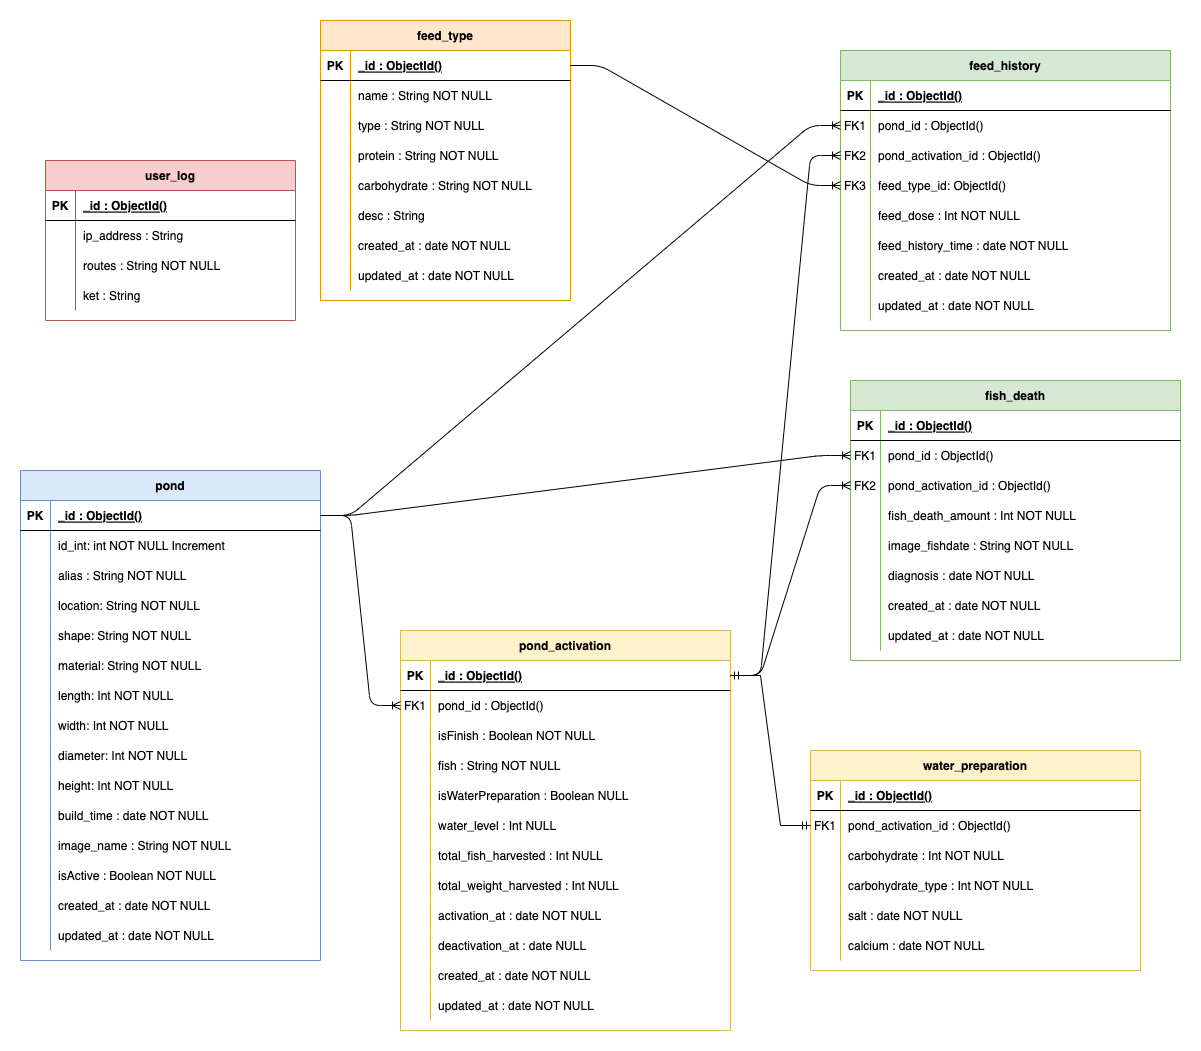
\includegraphics[height=0.7\textwidth]{gambar/Sprint05/diagram database/database}
	\caption{ERD Database Sprint-5}
	\label{fig:database_sprint5}
\end{figure}

Dengan berubahnya desain database diperlukan juga penambahan model pada source code, berikut perubahan pada source code model.

\begin{lstlisting}
# fishapi/database/model.py

class FishDeath(db.Document):
    pond_id = db.ReferenceField(Pond, required=True)
    pond_activation_id = db.ReferenceField(PondActivation, required=True)
    image_name = db.StringField(required=True)
    diagnosis = db.StringField(default=datetime.datetime.now)
    death_at = db.DateTimeField(default=datetime.datetime.now)
    created_at = db.DateTimeField(default=datetime.datetime.now)
    updated_at = db.DateTimeField(default=datetime.datetime.now)
\end{lstlisting}




\item \textbf{Implementasi API entry kematian ikan}

Implementasi controller API entry kematian ikan, berikut merupakan perubahan source code controller API entry kematian ikan.

\begin{lstlisting}
# fishapi/database/fishdeath.py

class PondActivationApi(Resource):
    def post(self):
        try:
            pond_id = request.form.get("pond_id", None)
            pond = Pond.objects.get(id=pond_id)
            if pond.isActive == False:
                response = {"message": "status pond is not active"}
                response = json.dumps(response, default=str)
                return Response(response, mimetype="application/json", status=400)
            pond_activation = PondActivation.objects(
                pond_id=pond_id, isFinish=False).order_by('-activated_at').first()
            try:
                file = request.files['image', None]
                if not allowed_file(file.filename):
                    response = {"message": "file type not allowed"}
                    response = json.dumps(response, default=str)
                    return Response(response, mimetype="application/json", status=400)
                filename = secure_filename(file.filename)
                filename = pad_timestamp(filename)
                path = os.path.join(current_app.instance_path,
                                    current_app.config['UPLOAD_DIR'])
                try:
                    os.makedirs(path)
                except OSError:
                    pass
                filepath = os.path.join(path, filename)
                file.save(filepath)
            except:
                filename = "default.jpg"
            fish_death_amount = request.form.get("fish_death_amount", "[]")
            fish_death_amount = json.loads(fish_death_amount)
            if len(fish_death_amount) < 1:
                response = {"message": "There is no fish"}
                response = json.dumps(response, default=str)
                return Response(response, mimetype="application/json", status=400)
            body = {
                "pond_id": pond.id,
                "pond_activation_id": pond_activation.id,
                "image_name": filename,
                "diagnosis": request.form.get("diagnosis", None),
            }
            fishdeath = FishDeath(**body).save()
            id = fishdeath.id
            for fish in fish_death_amount:
                # save fish log
                data = {
                    "pond_id": pond_id,
                    "pond_activation_id": pond_activation.id,
                    "fish_death_id": id,
                    "type_log": "death",
                    "fish_type": fish['type'],
                    "fish_amount": int(fish['amount']) * -1
                }
                fishlog = FishLog(**data).save()
            response = {"message": "success add fishdeath"}
            response = json.dumps(response, default=str)
            return Response(response, mimetype="application/json", status=200)
        except Exception as e:
            response = {"message": str(e)}
            response = json.dumps(response, default=str)
            return Response(response, mimetype="application/json", status=400)
\end{lstlisting}

Kode ini adalah sebuah fungsi yang menangani permintaan POST yang dikirimkan ke server.

Pertama, fungsi ini mencoba untuk mengambil nilai "pond\_id" dari permintaan yang diterima. Jika nilai ini tidak ada, maka nilai "pond\_id" akan diatur menjadi None. Kemudian fungsi mencoba untuk mendapatkan objek Pond dari database dengan menggunakan nilai "pond\_id" yang diperoleh sebelumnya.

Jika nilai isActive dari objek Pond adalah False, maka fungsi akan mengembalikan pesan kesalahan dengan kode status 400. Jika nilai isActive adalah True, maka fungsi akan mencoba mendapatkan objek PondActivation dengan menggunakan nilai "pond\_id" yang diperoleh sebelumnya. Objek PondActivation yang diperoleh akan memiliki isFinish=False dan diurutkan berdasarkan tanggal aktivasi terbaru.

Selanjutnya, fungsi akan mencoba untuk mendapatkan file gambar dari permintaan yang diterima. Jika jenis file tidak diizinkan, maka fungsi akan mengembalikan pesan kesalahan dengan kode status 400. Jika jenis file diizinkan, maka fungsi akan menyimpan file gambar di dalam direktori yang ditentukan.

Setelah itu, fungsi akan mencoba untuk mengambil nilai "fish\_death\_amount" dari permintaan yang diterima dan mengonversinya menjadi objek Python. Jika nilai "fish\_death\_amount" kosong, maka fungsi akan mengembalikan pesan kesalahan dengan kode status 400.

Kemudian, fungsi akan membuat objek FishDeath dengan menggunakan nilai-nilai yang diperoleh sebelumnya, dan menyimpannya ke dalam database. Fungsi juga akan membuat objek FishLog untuk setiap jenis ikan yang tercatat mati, dan menyimpannya ke dalam database.

Terakhir, fungsi akan mengembalikan pesan sukses dengan kode status 200, atau pesan kesalahan dengan kode status 400 jika terjadi kesalahan selama proses. Semua pesan yang dikirimkan dalam format JSON.

Terakhir, fungsi mengembalikan respons dalam format JSON yang berisi pesan berhasil atau gagalnya aktivasi kolam.

Berikut merupakan form untuk entry musim budidaya.

\begin{longtable}{| l | p{5cm} | p{5cm} |}
\caption{Form entry kematian ikan.\label{table:form_entry_kematian_ikan}}\\

\hline
\multicolumn{1}{|c|}{\textbf{Form}} & \multicolumn{1}{|c|}{\textbf{Jenis Data}} & \multicolumn{1}{|c|}{\textbf{Deskripsi}}\\
\hline
\endfirsthead

\hline
\multicolumn{3}{|c|}{Lanjutan Tabel \ref{table:form_entry_kematian_ikan}}\\
\hline
\multicolumn{1}{|c|}{\textbf{Form}} & \multicolumn{1}{|c|}{\textbf{Jenis Data}} & \multicolumn{1}{|c|}{\textbf{Deskripsi}}\\
\hline
\endhead

                                          

pond\_id            & REQUIRED STRING                                                                                                                                             & id kolam yang mengalami kematian ikan \\ \hline
fish\_death\_amount & REQUIRED JSON FISH TYPE: {[}"nila hitam", "nila merah", "lele", "patin", "mas",{]} Ex: {[}\{"type": "lele","amount": 5\},\{"type": "patin","amount": 9\}{]} & tipe dan banyak ikan                  \\ \hline
image               & OPTIONAL FILE                                                                                                                                               & foto kematian ikan                    \\ \hline
diagnosis           & REQUIRED STRING                                                                                                                                             & diagnosa kematian ikan                \\ \hline

\end{longtable}


Tabel tersebut merupakan deskripsi dari jenis data yang diperlukan pada form untuk menambahkan data kematian ikan pada suatu kolam. Form ini meminta input berupa pond\_id yang merupakan string yang mengacu pada id kolam yang mengalami kematian ikan. Selain itu, input fish\_death\_amount juga diperlukan dalam bentuk JSON dengan jenis data yang terdiri dari "nila hitam", "nila merah", "lele", "patin", dan "mas". Fish\_death\_amount menyimpan informasi tentang jenis dan banyaknya ikan yang mati. Input file image bersifat opsional dan meminta foto kematian ikan, sedangkan diagnosis yang diperlukan dalam bentuk string merujuk pada diagnosa kematian ikan.

Berikut merupakan hasil test request dari API entry kematian ikan.

cURL:

\begin{lstlisting}
curl --location 'http://jft.web.id/fishapi/api/fishdeath' \
--form 'pond_id="625d7026a9a73e090c65cda1"' \
--form 'fish_death_amount="[{\"lele\": 10},{\"patin\":20}]"' \
--form 'image=@"/Users/andrirahmanto/Downloads/Mass-fish-death-Menindee.jpeg"' \
--form 'diagnosis="mati karena sakit"'
\end{lstlisting}

response json:

\begin{lstlisting}
{
  "message": "success add fishdeath",
  "id": "62b9adfa793e0f39dbaa1739"
}
\end{lstlisting}




\item \textbf{Implementasi API edit kematian ikan}

Implementasi controller API edit kematian ikan, berikut merupakan perubahan source code controller API edit kematian ikan.

\begin{lstlisting}
# fishapi/database/fishdeath.py

def put(self, id):
        try:
            body = request.form.to_dict(flat=True)
            FishDeath.objects.get(id=id).update(**body)
            response = {"message": "success change data fish death", "id": id}
            response = json.dumps(response, default=str)
            return Response(response, mimetype="application/json", status=200)
        except Exception as e:
            response = {"message": str(e)}
            response = json.dumps(response, default=str)
            return Response(response, mimetype="application/json", status=400)
        return
\end{lstlisting}

Kode ini merupakan fungsi untuk mengubah data kematian ikan pada database. Fungsi ini menggunakan HTTP method PUT dan menerima parameter id, yang merupakan id dari data kematian ikan yang ingin diubah.

Pada blok try, terdapat dua baris kode. Baris pertama mengubah data request.form menjadi dictionary yang disimpan dalam variabel body. Baris kedua memanggil fungsi update pada model FishDeath dengan mengirimkan id dan dictionary body sebagai parameter.

Jika proses berhasil, akan mengembalikan response dengan status 200 dan message "success change data fish death" beserta id dari data yang diubah. Jika terjadi error, maka akan mengembalikan response dengan status 400 dan message error yang muncul pada variabel e yang diubah menjadi string.

Blok terakhir menggunakan return untuk mengakhiri fungsi.

Berikut merupakan form untuk edit kematian ikan.

\begin{longtable}{| l | p{5cm} | p{5cm} |}
\caption{Form edit kematian ikan.\label{table:form_edit_kematian_ikan}}\\

\hline
\multicolumn{1}{|c|}{\textbf{Form}} & \multicolumn{1}{|c|}{\textbf{Jenis Data}} & \multicolumn{1}{|c|}{\textbf{Deskripsi}}\\
\hline
\endfirsthead

\hline
\multicolumn{3}{|c|}{Lanjutan Tabel \ref{table:form_edit_kematian_ikan}}\\
\hline
\multicolumn{1}{|c|}{\textbf{Form}} & \multicolumn{1}{|c|}{\textbf{Jenis Data}} & \multicolumn{1}{|c|}{\textbf{Deskripsi}}\\
\hline
\endhead

                                          

pond\_id            & REQUIRED STRING                                                                                                                                             & id kolam yang mengalami kematian ikan \\ \hline
fish\_death\_amount & OPTIONAL JSON FISH TYPE: {[}"nila hitam", "nila merah", "lele", "patin", "mas",{]} Ex: {[}\{"type": "lele","amount": 5\},\{"type": "patin","amount": 9\}{]} & tipe dan banyak ikan                  \\ \hline
diagnosis           & OPTIONAL STRING                                                                                                                                             & diagnosa kematian ikan                \\ \hline

\end{longtable}


Tabel ini adalah deskripsi dari form edit kematian ikan dan memiliki tiga kolom yaitu Form, Jenis Data, dan Deskripsi.

Form menjelaskan nama dari field input pada form, Jenis Data menjelaskan tipe data dari field input, sedangkan Deskripsi memberikan penjelasan singkat mengenai deskripsi dari field input tersebut.

Pada tabel ini, terdapat 3 field input yaitu pond\_id, fish\_death\_amount, dan diagnosis. Kolom Jenis Data menunjukkan apakah field input tersebut merupakan tipe data REQUIRED STRING atau OPTIONAL JSON FISH TYPE dan Deskripsi memberikan penjelasan mengenai field input tersebut.

Field pond\_id wajib diisi dan berisi id kolam yang mengalami kematian ikan, sedangkan field fish\_death\_amount dan diagnosis bersifat opsional. Field fish\_death\_amount berisi tipe dan banyak ikan yang mati dan ditulis dalam format JSON, sedangkan field diagnosis berisi diagnosa kematian ikan.
Berikut merupakan hasil test request dari API entry kematian ikan.

cURL:

\begin{lstlisting}
curl --location -g --request PUT 'http://jft.web.id/fishapi/api/fishdeath/{fishdeath_id}' \
--form 'fish_death_amount="[{\"lele\": 10},{\"patin\":20}]"' \
--form 'diagnosis="mati karena sakit"'
\end{lstlisting}

response json:

\begin{lstlisting}
{
  "message": "success change data fish death",
  "id": "62b9adfa793e0f39dbaa1739"
}
\end{lstlisting}









\end{enumerate}